% This work is licensed under the Creative Commons Attribution-NonCommercial 4.0 International License.
% To view a copy of this license, visit http://creativecommons.org/licenses/by-nc/4.0/
% or send a letter to Creative Commons, PO Box 1866, Mountain View, CA 94042, USA.

% !TEX TS-program = xelatex

\documentclass[../Main/notes.tex]{subfiles}

\setcounter{chapter}{9}
\begin{document}

\chapter{Thermochemistry}

In this chapter we will discuss all the ingredients that are required to make accurate predictions of energy difference and transition barriers.
We will talk about how to reduce the errors in computations and the additional corrections that we can include and those that are typically neglected.

\section{How accurate is accurate enough?}
One of the major applications of computational chemistry is the prediction of energy differences, in particular for chemical reactions.
In this chapter we will analyze some of the most important contributions to the energy that should be included beyond the total electronic energy that you get at the end of a computation.

However, before we look into how to achieve high accuracy, we should ask: \emph{What degree of accuracy should quantum chemistry computations aim to achieve?}
To answer this question we could reason about the type of information we may want to extract from a quantum chemistry computation.
For example, if we are interested in evaluating the ratio of the population of two conformers, we might want to know what level of accuracy is necessary to compute the correct order of magnitude of this number.
The probability that a molecule in thermal equilibrium is in a conformation with energy $E_i$ is proportional to $\exp(-E_i  / k_\mathrm{B} T)$, where $k_\mathrm{B} = 1.38066 \times 10^{-23}$ J/K is the Boltzmann constant. 
The ratio of the number two conformers with energies $E_i$ and $E_j$ is then equal to
\begin{equation}
\frac{N_i}{N_j} = e^{- (E_i - E_j) / k_\mathrm{B} T}
\end{equation}
Here we assume that there are only two relevant conformations, and this equation needs to be modified for more general cases.
\emph{At room temperature (298 K) and converting to energy per mole, one can express the ratio in base 10 as}
\begin{equation}
\frac{N_i}{N_j} = 10^{- (E_i - E_j) / 1.36 \text{ kcal/mol}}
\end{equation}
Suppose that our computed value of $E_i - E_j$, which we will indicate with $\tilde{E}_i - \tilde{E}_j$, contains errors due to the approximations we used.
We can write the approximate energy difference as $\tilde{E}_i - \tilde{E}_j = E_i - E_j + \epsilon$, where $\epsilon$ is the error.
Then the conformers ration we compute is
\begin{equation}
\frac{\tilde{N}_i}{\tilde{N}_j} = 10^{- (\tilde{E}_i - \tilde{E}_j) / 1.36 \text{ kcal/mol}} = 10^{- (E_i - E_j + \epsilon) / 1.36 \text{ kcal/mol}}
= \frac{N_i}{N_j} 10^{-  \epsilon / 1.36 \text{ kcal/mol}}
\end{equation}
This simple computation shows that an error equal to 1.36 \kcal introduces an error in the predicted ration of a factor 10.
Therefore, if we want to compute the relative population within an order of magnitude from the true answer energy computations need to achieve an \emph{error for the energy difference} that is less than 1.36 \kcal.
This in an important result because it tells us that what is not necessary to achieve an absolute energy error of 1.36 \kcal.
If errors in two different computations (e.g., arising from the use of a small basis, an incomplete or approximate treatment of electron correlation) cancel out, we can still achieve accurate predictions of relative populations.

The above argument also applies to the determination of reaction constants.
This is the case because the Arrhenius equation for the reaction constant $k$ of a reaction with activation energy $E_\mathrm{a}$ is given by 
\begin{equation}
k=A e^{-E_\mathrm {a} / k_\mathrm{B}  T}
\end{equation}
This equation is similar to the one that we encountered above and leads to estimating that an error of 1.36 \kcal in the activation energy gives a reaction rate that is within a factor of 10 from the correct answer.

In the quantum chemistry literature, an error of less than 1 \kcal is often referred to as \emph{chemical accuracy}.
This energy error is commonly used as a criterion for judging if a method can make predictions that are sufficiently accurate for applications in chemistry.

\section{Types of energy computations}
The accuracy of predictions made with quantum chemistry methods relies heavily on a systematic cancellation of errors.
One of the most challenging type of computation is the atomization energy of a molecule, defined as the difference between the sum of the energy of the isolated atoms (in their ground state) that form a molecule and the energy of a molecule.
For example, the atomization energy of \ce{CO2} is the change in energy for the reaction
\begin{equation}
\ce{CO2} \rightarrow \ce{C} + \ce{O} + \ce{O}
\end{equation}
These type of computations are difficult because the resulting molecules are open-shells and the electron have significantly rearranged going from the molecules to the isolated atoms.

Atomization energies (and dissociation energies) can be computed in two different ways:
\begin{enumerate}
\item By taking the energy difference of the energy of the \emph{isolated} atoms and the molecule at its equilibrium geometry. For example, for \ce{CO2} this approach corresponds to computing the energy difference
\begin{equation}
E(\ce{C}) + 2 E(\ce{O}) - E(\ce{CO2})
\end{equation}
\item By taking the energy difference of the energy of the dissociated molecule and the molecule at its equilibrium geometry. In this case, the computation on the dissociated molecule is done by computing the atoms together but placing them at a very far distance (say, greater than 100--1000 \AA{}).
In this approach one computes the difference
\begin{equation}
E(\ce{O} \cdots \ce{C} \cdots \ce{O}) - E(\ce{CO2})
\end{equation}
where $E(\ce{O} \cdots \ce{C} \cdots \ce{O})$ stands for the energy of two isolated O and one C atoms (one computation).
\end{enumerate}
Ideally, both methods should give the same result. However, since most atoms are open-shell species you cannot directly apply methods like DFT to compute the energy of $E(\ce{O} \cdots \ce{C} \cdots \ce{O})$.
Therefore, the first route is preferable, although you can still run into issues with the computation of the individual atoms.

In most cases, we are interested in describing reactions in which only a few bonds are broken and formed.
This situation is easier for quantum chemistry, because computing similar systems leads to better error cancellation.
Chemical reactions can be classified according to the type and number of bonds that are broken/formed.
A classification often used for organic reactions is
\begin{itemize}
\item \emph{Isogyric reactions}, which conserve the number of electron pairs.
For example, the dissociation reaction
\begin{equation}
\ce{H2O} \rightarrow \ce{H}^\cdot + \ce{OH}^\cdot
\end{equation}
is \emph{not isogyric} because the electron pair that corresponds to one of the O-H bonds is broken.
The following reaction for the decomposition of butane is isogyric because the number of pairs is preserved\mnote{
This example is taken from Wheeler, Houck, v. R. Schleyer, and Allen, \textit{J. Am. Chem. Soc.} 2009, \textbf{131}, 2547.}

\begin{center}

\includegraphics[width=3.25in]{img/isogyric.png}
\end{center}

\item \emph{Isodesmic reactions}, which conserve the number of bonds and their type (the number of C-C bonds, C=C bonds, C-H bonds, etc.).
The following reaction is isodesmic because the three C-C bonds and 18 C-H bonds are preserved

\begin{center}

\includegraphics[width=3.25in]{img/isodesmic.png}
\end{center}

\item \emph{Homodesmotic reactions}, which conserve the number of bonds and the hybridized bond types (the number of sp$^3$-sp$^3$ C-C bonds, sp$^3$-H C-H bonds, etc.).
For example, this reaction preserves the number of sp$^3$-sp$^3$ C-C bonds (4) and contains an equal number of sp$^3$ C atoms with 3 hydrogens attached (4) and sp$^3$ C atoms with 2 hydrogens attached (2)

\begin{center}

\includegraphics[width=3.35in]{img/homodesmotic.png}
\end{center}

\end{itemize}
Computations performed on these three type of reactions are progressively more accurate because more features are conserved when going from the reactant to the products and there is better error cancellation.

\section{Basis set incompleteness}
One of the most obvious source of errors in quantum chemistry computations is due to the use of incomplete basis sets.
This error has been discussed in the chapter on basis sets.
Here we are interested in discussing how this error depends on the method and what procedures can be used to reduce it.

An important distinction is between methods like HF and DFT vs. correlated wave function methods like MP2, CCSD, and CCSD(T).
In the case of HF and DFT, when one uses a systematic basis the energy error due to basis set incompleteness \emph{decays exponentially} with the highest angular momentum of a basis.
This means that the energy error is proportional to $\exp(-\beta X)$, where $X$ is the maximum angular momentum of a basis.
Therefore, moderately large basis sets (triple or quadruple zeta) are already sufficient to achieve well converged energies (with respect to the basis).
For correlated wave function methods, the convergence of the energy is instead \emph{polynomial}, approximately proportional to $X^{-3}$.
This error decays significantly slower than in the case of DFT, and in practice it means that very large bases are needed to converge the energy of correlated wave function methods.

\mfigure{
\captionof{table}{Convergence of the fragmentation energy (in \kcal) of NCCO to CN + CO. Each column shows the contribution going from the previous level of theory to the next one.}
\begin{tabular}{@{} lcrr @{}}
\toprule
Basis & HF & CCSD & CCSD(T) \\
\midrule
cc-pVDZ & +20.31 & −7.93 & +0.49 \\
cc-pVTZ & +20.87 & −7.55 & +0.74 \\
cc-pVQZ & +20.62 & −7.44 & +0.84 \\
cc-pV5Z & +20.71 & −7.41 & +0.88 \\
cc-pV6Z & +20.71 & −7.38 & +0.89 \\
CBS limit & +20.71 & −7.35 & +0.90 \\
\bottomrule
\end{tabular}
\label{fig:thermo:ncco}
}

A simple way to reduce the basis set incompleteness error is to fit an energy expression to computations with finite basis sets and then \emph{extrapolate the energy} to the limit $X \rightarrow \infty$.
In the case of Hartree--Fock theory, this can be done by fitting the energy to the form
\begin{equation}
E_\mathrm{HF}(X) = E_\mathrm{HF}(\infty) + \alpha \exp(-\beta X)
\end{equation}
This equation has three unknowns: 1) the complete basis set energy $E(\infty)$, and the two constants $\alpha$ and $\beta$.
Therefore it is necessary to perform three computations to extrapolate this energy.
A simpler form exist, where the value of $\beta$ is assumed to be a constant, and that requires only two energy computations.
In the case of correlated methods, one fits the energy increment due to correlation (the correlation energy), and this quantity is fitted to the equation
\begin{equation}
E_\mathrm{corr}(X) = E_\mathrm{corr}(\infty) + \alpha X^{-3}
\end{equation}


Table~\ref{fig:thermo:ncco} shows the convergence of various contributions to the total energy for basis sets of increasing size and the results obtained by extrapolating the energies.
Note that the HF contribution computed with the cc-pVTZ basis is only 0.16 \kcal away from the complete basis set (CBS) limit.
The combined contribution from CCSD and CCSD(T) computed with the same basis differs from the CBS answer by 0.36 \kcal.
When using a cc-pV5Z basis, the HF energy is converged to the CBS limit, while the contribution from the correlation energy is still 0.08 \kcal off.


A more sophisticated to reduce the dependency of the correlation with respect to $X$ is to use \emph{explicitly correlated methods}. These are modified versions of MP2, CCSD, CCSD(T), etc. that explicitly include terms in the wave function that depend on the interelectronic distance $r_{12} = | \mathbf{r}_1 - \mathbf{r}_2|$. These methods have a basis set error that scales approximately as $X^{-7}$
This class of $r_{12}$ methods is implemented in only a few quantum chemistry codes because of the added complexity required by the extra terms.

\section{Treatment of the correlation energy}

\mfigure{
\centering{
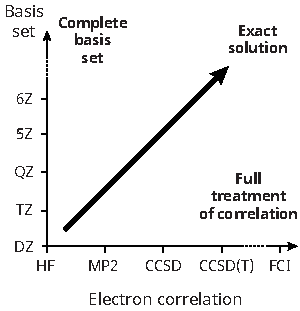
\includegraphics[width=2.00in]{img/focalpoint.pdf}
}
\captionof{figure}{To reach the exact solution of the (electronic) Schr\"{o}dinger equation it is necessary to simultaneously improve both the quality of the basis set (by including more basis functions) and the treatment of the correlation energy (for example, by including higher excited determinants).}
\label{fig:thermo:highaccuracy}
}

The second most important aspect to consider when aiming to achieve high accurate computational results is electron correlation.
Correlated methods offer a natural hierarchy to converge computations towards the exact limit (FCI).
However, it is important to note that the exact solution to the Schr\"{o}dinger can be achieved only by improving both the basis and the treatment of correlation effects.
This point is illustrated in Fig.~\ref{fig:thermo:highaccuracy}.

To converge the correlation energy towards the FCI limit, it is common to employ coupled cluster methods.
One way to monitor the convergence toward the exact solution is to perform computations at different level of theory and compare the \emph{increment} in the energy or any other target property from one level to the next.
For highly-accurate (sub-\kcal) one must include up to quadruple excitations in the coupled cluster treatment, which often done by performing the following series of computations
\begin{equation}
\text{HF} \rightarrow \text{MP2} \rightarrow \text{CCSD} \rightarrow \text{CCSD(T)} \rightarrow \text{CCSDT} \rightarrow \text{CCSDT(Q)}
\end{equation}

In the case of DFT computations there is no systematic way to improve an answer and the best pragmatic approach is to use functionals that have been extensively benchmarked.

\section{Vibrational corrections and entropic terms}

\mfigure{
\centering{
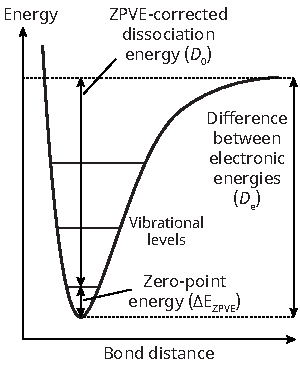
\includegraphics[width=2.00in]{img/zpve}
}
\captionof{figure}{Dissociation curve for a diatomic molecule. The dissociation energy corrected for the zero-point energy ($D_0$) is the difference between the energy of the dissociated molecule and the energy of the ground vibrational level.}
\label{fig:thermo:zpve}
}

Up to this point we have only considered how to improve the approximation of the electronic wave function.
An important class of corrections to the energy that should be included in computations of the thermodynamic properties of molecules should include \emph{corrections due to the zero-point vibrational energy (ZPVE)}.
Vibrational corrections account for the energy of the nuclei.
In the Born--Oppenheimer approximation this energy is computed separately by solving the nuclear Schr\"{o}dinger equation.

Figure~\ref{fig:thermo:zpve} shows the importance of zero-point vibrational corrections for the case of a diatomic molecule.
When computing the dissociation energy it is important to keep into account the fact that the energy of the molecule is not the bottom of the potential energy well, which corresponds to the electronic energy, the energy of the electrons alone.
The correct energy is the bottom of the well energy plus the zero-point vibrational energy.
In the case of the dissociated molecule, the ZPVE is zero (because the nuclei have zero kinetic energy) and so the energy contains only the electronic contribution.
ZPVE corrections to the dissociation energy of a bond can be of the order of one \kcal and can play an important role if there are significant molecular rearrangements in a reaction.

As we have seen before, one approximate solution to the nuclear Schr\"{o}dinger equation is based on the assumption that nuclei vibrate around their equilibrium positions in a quadratic potential (harmonic approximation).
This computation is routinely performed when computing the vibrational frequency of a molecule.
As we have seen before, the ZPVE correction in the harmonic approximation is given by
\begin{equation}
\label{eq:thermochemistry:zpve}
E_0 = V_0 + \frac{1}{2}  \sum_{v_\alpha} \omega_\alpha
\end{equation}
where $\omega_\alpha$ is the energy spacing between vibrational levels for the normal mode $\alpha$ (this quantity is related to the vibrational frequency of a normal mode).

\mfigure{
\centering{
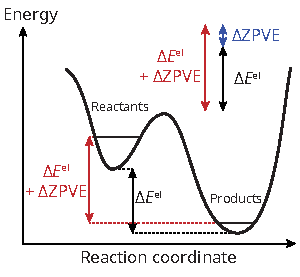
\includegraphics[width=2.00in]{img/zpve2}
}
\captionof{figure}{Under the Born--Oppenheimer approximation, the change in energy in a reaction is the sum of the electronic energy difference ($\Delta E^\text{el}$) and the change in zero-point vibrational energy ($\Delta \text{ZPVE}$).}
\label{fig:thermo:zpve2}
}

When computing the energy change for a reaction one need to account for the ZPVE for both the reactant and products.
This point is illustrated in Fig.~\ref{fig:thermo:zpve2}, where we consider the case of a reaction that proceeds via a transition state in one dimension.
The change in energy corresponding to this reaction is given by the sum of the electronic energy difference ($\Delta E^\text{el}$) plus the difference between the zero-point vibrational energies ($\Delta \text{ZPVE}$)
\begin{equation}
\Delta E = E_\text{prod} - E_\text{react} = 
\underbrace{E^\text{el}_\text{prod} - E^\text{el}_\text{react}}_{\Delta E^\text{el}}
+ \underbrace{\text{ZPVE}_\text{prod} - \text{ZPVE}_\text{react}}_{\Delta \text{ZPVE}}
\end{equation}
In the case of transition state computations, one of the vibrational frequencies is imaginary. \emph{This mode is excluded from the computation of the ZPVE correction for the transition state}.

Once the vibrational frequencies are known, it is possible to compute various thermodynamic properties.
Since at finite temperature a population of non-interacting molecule in the gas phase is vibrationally, rotationally, and translationally excited (according to the Boltzmann distribution) there are thermal corrections for each of these contributions.
For example, psi4 defines the internal (thermal) energy $U(T)$ as the sum of the electronic energy, the ZPVE, and vibrational, rotational, and translational energies
\begin{equation}
U(T) = E^{\mathrm{el}} + E^{\mathrm{ZPVE}}
+ E^{\mathrm{vib}} + E^{\mathrm{rot}} + E^{\mathrm{trans}}
\end{equation}
This energy depends on the temperature and it is usually computed at 298.15 K.
At $T  = 0 $ K the internal energy is equal just to the sum of the electronic and ZPVE
\begin{equation}
U(0) = E^{\mathrm{el}} + E^{\mathrm{ZPVE}}
\end{equation}
\emph{Quantum computational studies typically report both the electronic energy $ E^{\mathrm{el}}$ and the ZPVE corrected value $E^{\mathrm{el}} + E^{\mathrm{ZPVE}}$.}

A frequency computation also provides values for the \emph{enthalpy} [$H = U + pV$] and the \emph{Gibbs free energy} [$G = H - TS$].
The enthalpy corresponds to the heat adsorbed or emitted in a reaction under constant pressure.
This quantity is used to compute reaction enthalpies and enthalpies of formation of molecules.
The free energy accounts for both the change in enthalpy and entropy and it can be used to characterize whether or not a process is spontaneous ($\Delta G < 0$).

There are two important point to remember: 1) Thermodynamical corrections are computed using the harmonic approximation, and 2) that a computation yields the absolute value of these quantities.
A note of caution is important. From the Psi4 manual:
\begin{quote}
 It is important to know that Psi4, like any other quantum chemistry program, does \textit{not} compute the usual enthalpies, entropies, or Gibbs free energies of \textit{formation} provided by most reference books. Instead, quantum chemistry programs compute “absolute” thermodynamic properties relative to infinitely separated nuclei and electrons, not “formation” values relative to elements in their standard states. If you are computing thermodynamic differences, like a reaction enthalpy computed as the enthalpy of the products minus the enthalpy of the reactants, then these “absolute” enthalpies are perfectly valid and usable. However, they cannot be mixed and matched with enthalpies of formation from reference books, since the zero of energy is not the same.
\end{quote}


The ZPVE correction computed via Eq.~\eqref{eq:thermochemistry:zpve} is based on the approximation that the potential energy experienced by nuclei is quadratic.
To improve upon this approximation one can consider \emph{anharmonicity corrections}.
These are important both to predict better thermodynamics and spectroscopic properties.
Anharmonicity corrections take into account deviations of the potential energy from the quadratic approximations, and therefore require evaluating third and higher derivatives of the energy.
The simplest form of anharmonic corrections are obtained by applying vibrational  second-order perturbation theory (VPT2).

\section{Smaller terms: Corrections to the Born--Oppenheimer approximation and relativistic effects}

The last two sources of errors arise from approximations in the Hamiltonian.
As we have seen in the early chapters, the Born--Oppenheimer or fixed nuclei approximation is one of the first simplifications made when solving the Schr\"{o}dinger equation for atoms and molecules.
The BO approximation is most effective when the ratio between the electrons and nuclei, $m_e / M_i$ is small.
This ratio has the largest value for the hydrogen atom ($m_e / M_i \approx 1/1836$) since it is the lightest nucleus.
In most cases, the BO approximation is extremely accurate and there is no need to compute corrections.
However, there are problems in chemistry where the BO breaks down.
This is the case especially when the electronic and nuclear degrees of freedom in a molecule are strongly coupled (e.g. proton-coupled electron transfer).

For most of the chemistry of the first 2-3 rows of the periodic table (H--Ar), relativistic effects play a negligible or small role.
Therefore, the effects of relativity are typically ignored.
However, relativistic effects gradually become more important as we move to nuclei with larger nuclear charge and can have make a significant difference in the physical/chemical properties of elements.\mnote{Famous examples are the color of gold (predicted to be gray when relativistic effects are ignored) and the low melting temperature of mercury.}

Relativistic effects can be separated into scalar relativistic effects (independent of spin) and spin-orbit effects.
Scalar effects contribute to the contraction of the core electrons.
Spin-orbit effects instead couple the spin of the electrons with the angular momentum of electrons, and are particularly important for open-shell species.
The simplest way to treat scalar relativistic effects is via \emph{effective core potentials (ECPs)}.
These are fictitious potentials that replace the contribution from core electrons and are parameterized to account for the most important relativistic corrections.
Another route consists in solving the \emph{Dirac equation}, the relativistic equivalent of the Schr\"{o}dinger equation.
The Dirac equation describes both electrons and positrons and it is considerably more challenging to solve than the nonrelativistic Schr\"{o}dinger equation.

\end{document}